\IEEEraisesectionheading{\section{Introduction}\label{sec:introduction}}

深度卷积神经网络(DCNNs) \cite{LeCun1998} 已经将计算机视觉系统在各种高级问题上的性能推向了历史新高, 包括图像分类 \cite{KrizhevskyNIPS2013, sermanet2013overfeat, simonyan2014very, szegedy2014going, papandreou2014untangling} 和 对象检测 \cite{girshick2014rcnn, erhan2014scalable, girshick2015fast, ren2015faster, he2015deep, liu2015ssd},其中 DCNNs 以端到端训练的方式完胜传统的人工特征提取,取得了惊人的效果。

DCNNs 成功的关键在于它们对局部图像变换的内置不变性,这使它们能够学习越来越抽象的数据表示 \cite{zeiler2014visualizing}。这种不变性对于分类任务显然是可取的,但是对于像素级敏感的、密集的预测任务不尽然,例如语义分割,其中空间信息的抽象是不希望看到的。

特别地,我们考虑将 DCNNs 应用于图像语义分割任务中的以下三个挑战:(1)降低的特征分辨率,(2)存在多尺度变化下的物体,以及(3)由于 DCNNs 不变性而导致的定位精度下降。接下来,我们将讨论这些挑战及在我们提出的 DeepLab 系统中克服它们的方法。

第一个挑战是由最初为图像分类设计的多级最大池化及下采样(stride)操作组合引起的 \cite{KrizhevskyNIPS2013, simonyan2014very, szegedy2014going}。当 DCNNs 以完全卷积方式计算时,计算出的特征图的分辨率显著下降 \cite{long2014fully}。为了克服这一障碍并有效生成更为密集的特征,我们从 DCNNs 的最后几个最大池化层中移除了下采样操作,并在后续的卷积层中使用上采样滤波器,从而以更高的采样率计算特征。上采样滤波器相当于在非零滤波器的感受野中插入了许多空洞。这项技术在信号处理领域有着悠久的历史,最初是用来计算小波变换的 \cite{holschneider1989real}。我们借用了术语 \textit{空洞卷积} 作为使用上采样滤波器卷积的缩写。已经有不少 DCNNs 曾使用了这一技术并发表了文章 \cite{giusti2013fast, sermanet2013overfeat, papandreou2014untangling}。在实践中,我们通过结合空洞卷积来恢复全分辨率特征图,这种卷积方法更加密集地计算了特征图,接着对特征图做简单的双线性插值运算,恢复到了原图的大小。此方法提供了在密集预测任务中使用反卷积 \cite{zeiler2014visualizing, long2014fully} 的一种简单而强大替代方法。与具有较大滤波器的常规卷积相比,空洞卷积允许我们有效地扩大滤波器的感受野而不增加参数的数量或计算量。

第二个挑战是由存在多个尺度的物体引起的。处理这一问题的标准做法是向 DCNNs 输入同一图像的不同缩放版本,然后聚合特征图或分数图 \cite{papandreou2014untangling, chen2015attention,kokkinos2016pushing}。我们验证了这种方法的确能提升精度,但是对应一张图片要以其所有缩放版本的计算量为代价。然而,在空间金字塔池化方法 \cite{lazebnik2006beyond, he2014spatial} 的帮助下,我们使用了一种高效的计算方案,在进行卷积之前,以多种采样率重新采样给定的特征图。这相当于使用多个具有互补感受野的滤波器去处理原始图像,从而捕获物体及多个尺度下的图像上下文。我们使用多个并行的、具有不同采样率的空洞卷积,而不是真正地重新采样特征。这种组合技术我们称之为 ``\textit{空洞空间金字塔池化}''(ASPP)。

第三个挑战涉及到这样一个事实,即以物体为中心的分类器需要空间变换不变性,从而固有地限制了 DCNNs 的空间精度。减轻精度下降的一种方法是,在计算最终分割结果时使用跳跃层从多个网络结构中抽取 ``超列'' \cite{hariharan2014hypercolumns, long2014fully}。我们研究探索了一种非常有效的替代办法——通过采用完全连接的条件随机场来提高模型捕获精细细节的能力 \cite{krahenbuhl2011efficient}。CRF 已广泛用于语义分割,以将由多路分类器计算的类分数与由像素和边缘 \cite{rother2004grabcut, shotton2009textonboost} 或超像素 \cite{lucchi2011spatial} 的局部低级信息组合。尽管已经提出了增加复杂性的工作来模拟分割依赖性 \cite{he2004multiscale, ladicky2009associative, lempitsky2011pylon} 和(或)分段的高阶依赖性 \cite{delong2012fast, gonfaus2010harmony, kohli2009robust, CPY13, Wang15},但我们使用完全连接的成对 CRF 进行高效计算 \cite{krahenbuhl2011efficient},并且在捕获精细边缘细节同时也适应了长时间的范围依赖。在 \cite{krahenbuhl2011efficient} 中提出的模型提升了像素级分类器的性能。在这项工作中,我们证明当与基于 DCNNs 的像素级分类器结合使用时,它能产生出色的结果。

\begin{figure*}[!th]
  \centering
  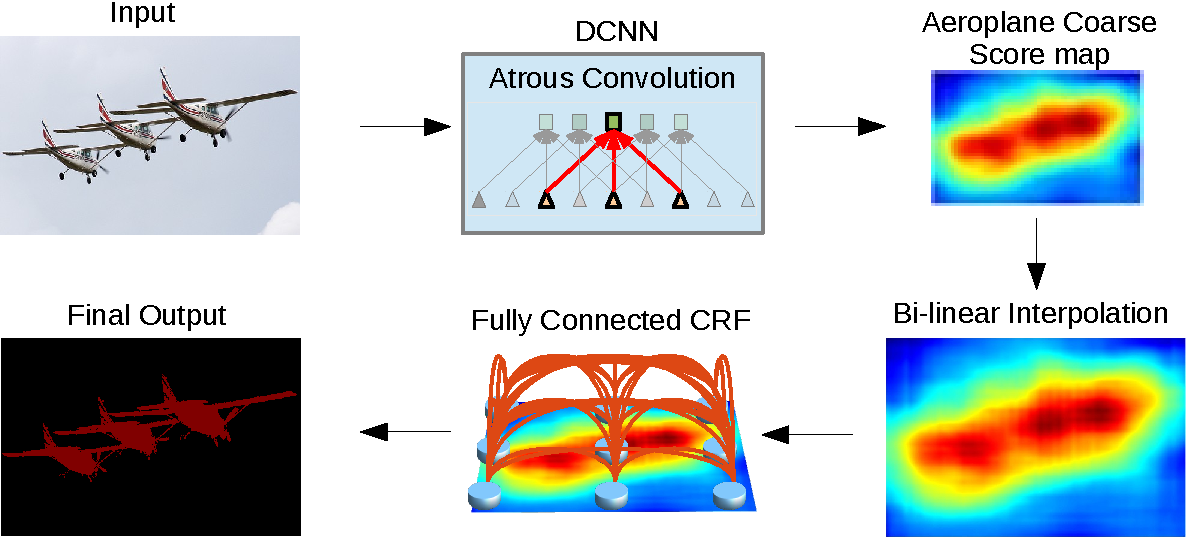
\includegraphics[width=0.7\linewidth]{fig/model_illustration4.pdf}
  \caption{模型图。诸如 VGG-16 或 ResNet-101 之类的 DCNNs 以完全卷积的方式使用,使用空洞卷积来降低信号下采样的程度(从32$\times$ 下降到 8$\times$)。双线性插值将特征放大到原始图像分辨率。然后使用完全连接的 CRF 来细化分割结并更好地捕获物体边界。} \label{fig:ModelIllustration}
\end{figure*}

\figref{fig:ModelIllustration} 展示了我们提出的 DeepLab 模型的高层结构。在图像分类任务中训练的深度卷积网络(VGG-16 \cite{simonyan2014very} 或 ResNet-101 \cite{he2015deep})通过以下方式重新运用于图像语义分割任务:(1)将所有全连接层换成卷积层 \cite{long2014fully},(2)通过空洞卷积层增加特征分辨率,使得我们能计算原图中每8个像素的特征而不是每32个。然后,我们采用双线性插值将分类分数图上采样 8 倍,以达到原图分辨率,从而产生全连接 CRF 的输入 \cite{krahenbuhl2011efficient},来达到细化分割结果的目的。

从实用的角度来看,我们的 DeepLab 系统有三大优点:(1)速度:由于空洞卷积的使用,我们的 DCNN 以 8 FPS 的速度在 NVidia Titan X GPU 上运行,全连接 CRF 的平均场推断在 CPU 上需要大约 0.5 秒;(2)精度:在众多图像分割数据集挑战中,我们的模型一举夺魁,包括 PASCAL VOC 2012 \cite{everingham2014pascal}, PASCAL-Context \cite{mottaghi2014role}, PASCAL-Person-Part \cite{chen_cvpr14} 以及 Cityscapes \cite{Cordts2016Cityscapes};(3)复杂度:我们的系统是由 DCNNs 和 CRFs 这两个非常成熟的模块级联组合而成的,便于理解和编写。

这篇论文中介绍的更新过的 DeepLab 与我们最初发表的第一个版本相比有几项改进 \cite{chen2014semantic}。新版本能够通过多尺度输入 \cite{farabet2013learning, lin2015efficient, chen2015attention} 或 ASPP 更好地分割多个尺度下的物体。我们通过调整最新的 ResNet \cite{he2015deep} 图像分类 DCNN 构建了 DeepLab 的残差网络变体,与基于 VGG-16 \cite{simonyan2014very} 的原始模型相比,拥有更优的语义分割性能。最后,我们对多种模型变体进行了更全面的实验评估,并报告了最新结果,不仅是 PASCAL VOC 2012,还有其他具有挑战性的任务。我们通过扩展 Caffe 框架 \cite{jia2014caffe} 实现了 DeepLab,并在 \url{http://liangchiehchen.com/projects/DeepLab.html} 开放了源代码及模型数据。
